\documentclass[a4paper,11pt,oneside]{scrreprt}
\usepackage[latin1]{inputenc}
\usepackage[english]{babel}
\usepackage{graphicx}
\usepackage{float}
\usepackage{geometry}
\geometry{verbose,a4paper,tmargin=25mm,bmargin=25mm,lmargin=15mm,rmargin=25mm}
\usepackage{paralist}

\usepackage{paracol}

\usepackage{todonotes}

\usepackage{listings}
\lstset{language=Java,
	tabsize=2,
	showspaces=false,
	showtabs=false,
	breaklines=true,
	showstringspaces=false,
	breakatwhitespace=true,
	commentstyle=\color{pgreen},
	keywordstyle=\color{pblue},
	stringstyle=\color{pred},
	basicstyle=\footnotesize\ttfamily,
	moredelim=[il][\textcolor{pgrey}]{$$},
	moredelim=[is][\textcolor{pgrey}]{\%\%}{\%\%}
}

\usepackage{tikz}
\usetikzlibrary{calc,patterns,angles,quotes}

\usepackage{caption}
\usepackage{subcaption}
\usepackage{tabularx} % in the preamble
\usepackage{pdfpages}
\usepackage{grffile}

\begin{document}


\begin{center}
	Submitted by Group 36
	
	\bigskip
	
	\begin{tabular}{c}
	Group Members: \\
	CETIN, Ulfet (391819); GRUCZKA, Filip (413279);	LIPINSKI, Bartosz (413177) \\
	\end{tabular}

	\bigskip
	
	DIS1 WS 19/20 Assignment 5\\
	Understanding the Evolution of Interface Design
	
	%	(ordered on lastname basis)
\end{center}


\noindent\fbox{%
	\parbox{\textwidth}{%
		\textbf{Feature \# : } 1 
		
		\textbf{Interface : } Put That There
		
		\textbf{Occurs at time : } 2:30
		
		\textbf{Description: } Objects such as sea vehicles storing their previous states (such as position or size), and being restored to their previous states just by giving `revert` command via speech.
		
		\par\noindent\rule{\textwidth}{0.4pt}
		
		\textbf{Comparison against current devices (or) technology:}
		
		\begin{compactitem}
			\item \textbf{Name of the current device or technology:} current UI designs \& interactions \\
			\textbf{Description:} YES (this feature does exist in current devices).
			We store the older states of objects in, for example, drawing programs, and we can restore it.
			
			However, it is different than before in a negative way.
			In the video, it is shown that it is done just by saying the name of the object, and issuing "make it what it was" command. Nowadays, we do not have voice recognition to point to the object and another voice command to rotate it. It is mostly with selection via other methods such as touching/pointing/clicking, and issuing a similar `revert` command via help of sound recognition or a keyboard.
		\end{compactitem}
	
		\bigskip 
		
		\hspace{8em}	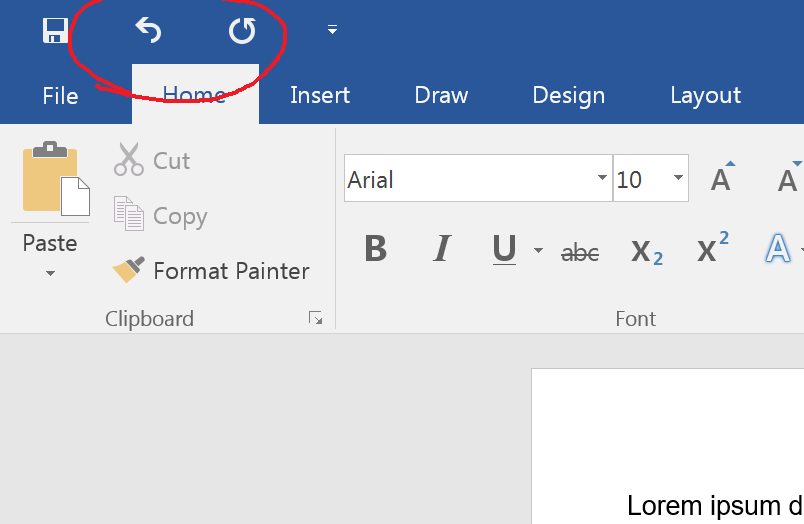
\includegraphics[clip, trim=0cm 5cm 0cm 0cm, scale=1.0]{../pics/1.png}
		
	}%
}

\bigskip
\noindent\fbox{%
	\parbox{\textwidth}{%
		\textbf{Feature \# : } 2
		
		\textbf{Interface : } Put That There
		
		\textbf{Occurs at time : } 3:30
		
		\textbf{Description: } Machine not recognizing a request in a complete sense, but still splitting command into two as `command` and `pointed object` and :
		" ?? (copy)" "THAT"
		Then only asking for the part that it did not manage to recognize: in our case, the `command` part is not recognized and the machine asks for clarification by saying "What command?", and not asking for the object again, as it recognized it already.
		
		\par\noindent\rule{\textwidth}{0.4pt}
		
		\textbf{Comparison against current devices (or) technology:}
		
		\begin{compactitem}
			\item \textbf{Name of the current device or technology:} none \\
			\textbf{Description:} NO (this feature does NOT exist in current devices).
			Although that we have devices such as Alexa from Amazon or similar gadgets from Google, those gadgets, in their current form, most of the time want the user to repeat the whole request, from its start to its end.
			
			It is not achieved yet, because the technology is behind it. How Alexa-like gadgets makes sense out of user requests is that they either make an educated guess if they do not fully recognize the request and this leads to user frustration, or they ask the user to repeat the request in its whole form again until it makes a sense to the said gadget. This is due to the fact that the speech recognition works in a contextual manner, and makes sense to the algorithm of the machine it is completely understood, as the lack of contextual information leads to many different speech recognition prediction and this makes it neigh impossible to make sense of the full request.
		\end{compactitem}
		
	}%
}

\bigskip
\noindent\fbox{%
	\parbox{\textwidth}{%
		\textbf{Feature \# : } 3
		
		\textbf{Interface : } Put That There
		
		\textbf{Occurs at time : } 2:43
		
		\textbf{Description: } Man pointing to objects \& interacting with objects via pointer device strapped to his wrist, and also have the cables of the pointing device going through his shirts' cuffs.
		
		\par\noindent\rule{\textwidth}{0.4pt}
		
		\textbf{Comparison against current devices (or) technology:}
		
		\begin{compactitem}
			\item \textbf{Name of the current device or technology:} Microsoft Kinect \\
			\textbf{Description:} NO (this feature does NOT exist in current devices)
			
			It could be argued that there are better current device features that cater to a similar purpose. A dedicated pointer capture (also seen in the video) and a dedicated pointer object  to wear, those things did not become mainstream most probably because they are cumbersome \& hard to wear, and to add, not so much portable. Instead of those, we have gesture and pointing recognizing technologies that\textbf{ do not} need a wearable device to operate. Those devices operate by recognizing the user's posture and hands by image recognition using cameras, and allows user to interact with objects without wearing a device that goes through their bodies via its cables. 
			
%			So, no need for a pointing device and a capture device capturing the pointing device's orientation nowadays, just image recognition to do the same functionality without the burden of two extra devices.
		\end{compactitem}
		
		\bigskip 
		
		\hspace{8em}	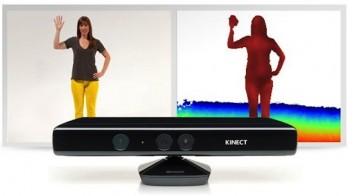
\includegraphics[clip, trim=0cm 0cm 0cm 0cm, scale=1.0]{../pics/3.jpg}
		
	}%
}

\bigskip
\noindent\fbox{%
	\parbox{\textwidth}{%
		\textbf{Feature \# : } 4
		
		\textbf{Interface : } Apple Knowledge Navigator
		
		\textbf{Occurs at time : } 2:44
		
		\textbf{Description: } Man is talking to maschine "copy the last 30 years at this location has one month intervals" and then he is inserting "credit card looking" pen drive to the machine.
		
		\par\noindent\rule{\textwidth}{0.4pt}
		
		\textbf{Comparison against current devices (or) technology:}
		
		\begin{compactitem}
			\item \textbf{Name of the current device or technology:} pen drives \\
			\textbf{Description:} NO (this feature does NOT exist in current devices)
			
			We do have pen drives and it is really common way to send information from the computer to the user portable device (and vice versa). 
			But the way of copying data is limited:
			\begin{compactenum}
				\item insert pen drive to the machine
				\item select files you want to copy
				\item copy
			\end{compactenum}
			We can programm some script which will copy files from certain directory after inserting the pendrive. But nowadays in mainstream usage we do not use advanced voice commands to copy files. Furthermore in the video man told voice command before even inserting the pendrive. So the machine has to remember voice command before even detecting pendrive. That is also not present in current technology.
		\end{compactitem}
		
	}%
}

\bigskip
\noindent\fbox{%
	\parbox{\textwidth}{%
		\textbf{Feature \# : } 5
		
		\textbf{Interface : } Sun Starfire
		
		\textbf{Occurs at time : } 00:14
		
		\textbf{Description: } Lady is starting video conference with other person just by verbally issuing a command.
		
		\par\noindent\rule{\textwidth}{0.4pt}
		
		\textbf{Comparison against current devices (or) technology:}
		
		\begin{compactitem}
			\item \textbf{Name of the current device or technology:} Skype \\
			\textbf{Description:} YES (this feature does exist in current devices).
			
			It is really common to communicate with other people using video conference. We are using for example Skype, so we are able to talk with somebody like "face to face", we can see the person in the front of us. To add, there are AI-enhanced helpers such as Alexa to directly understand verbal commands and start such a video conference session with as desired.
		\end{compactitem}
		
	}%
}


\bigskip
\noindent\fbox{%
	\parbox{\textwidth}{%
		\textbf{Feature \# : } 6
		
		\textbf{Interface : } Sun Starfire
		
		\textbf{Occurs at time : } 2:11
		
		\textbf{Description: } Lady is reading article with her friend and then she want to scan one page of the article. She told "let me scan it" and then she flipped around an article and put on the desk.
		
		\par\noindent\rule{\textwidth}{0.4pt}
		
		\textbf{Comparison against current devices (or) technology:}
		
		\begin{compactitem}
			\item \textbf{Name of the current device or technology:} Scanners \\
			\textbf{Description:} NO (this feature does NOT exist in current devices)
			
			In nowadays scanners we have to put a document in the right way (to have intended results). Then we have results in the computer. In video lady does not care where to locate document on the table. Despite this, she has the intended results. That is not present in current scaners. We have scanners exactly for a4, a3 documents for reason.
		\end{compactitem}
		
	}%
}

\bigskip
\noindent\fbox{%
	\parbox{\textwidth}{%
		\textbf{Feature \# : } 7
		
		\textbf{Interface : } Sun Starfire
		
		\textbf{Occurs at time : }  3:07
		
		\textbf{Description: } Lady in the video wants to create good 3D model. Her friend does it by selecting a man from a video and putting the texture on a 3D model.
		
		\par\noindent\rule{\textwidth}{0.4pt}
		
		\textbf{Comparison against current devices (or) technology:} 
		
		\begin{compactitem}
			\item \textbf{Name of the current device or technology:} e.g. NBA 2K15 face scan \\
			\textbf{Description:} Yes (this feature does exist in current devices) 
		     
          This feature is used but in slightly different way. Nowadays it is not used in presentation programs (e.g. Power Point). However, it is used in computer games. In those games, computer player have a possibility to make game character look like him by scanning his face from a photo (similiar to that what a women in a video did with a car commercial). Game than processes a photo and puts it on game character. Games that use this feature are for example FIFA or NBA 2K, so it is quite popular technology today. The difference between video and present day is that you can scan only your face (scanning whole body is also possible, but it is not in commercial use).
		\end{compactitem}
		
	}%
}


\bigskip
\noindent\fbox{%
	\parbox{\textwidth}{%
		\textbf{Feature \# : } 8
		
		\textbf{Interface : } Apple Knowledge Navigator
		
		\textbf{Occurs at time : } 2:50
		
		\textbf{Description: } Flashing icon when the man connected device to a computer 
		
		\par\noindent\rule{\textwidth}{0.4pt}
		
		\textbf{Comparison against current devices (or) technology:}
		
		\begin{compactitem}
			\item \textbf{Name of the current device or technology:} Windows \\
			\textbf{Description:} Yes (this feature does exist in current devices)
			
			In current operating systems, if we connect some device to the computer, the icon of it appears on screen. For example - if we connect a printer, a printer-like icon shows up in the bottom bar on the screen. That informs user that the device is connected (or not) and allows him to use device's features, by clicking on an icon. The only difference between video and present day is that a user said to computer to copy something on a device before he had connected it, while currently, in most cases, user has to connect device first. 
		\end{compactitem}
		
	}%
}
\end{document}
